---
id: tkz-euclide-ejemplo-56
title: "Triángulo isósceles recto"
description: "Creación de un triángulo isósceles recto"
keywords: [angulo,triangulo,isosceles,recto,taller2]
tags: [tkzDefTriangle,tkzMarkSegments,tkzMarkAngles,tkzFillAngles,tkzDrawPolygon]
sort: 56
---
\documentclass[tikz,border=2mm]{standalone}
\usepackage{tkz-base}
\usepackage{tkz-euclide}

\begin{document}
    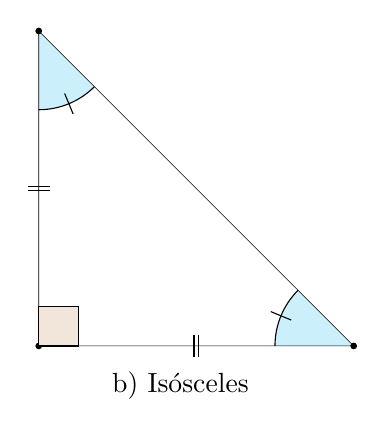
\begin{tikzpicture}
        % Paso 1: Define los puntos del triángulo △DEF
        \tkzDefPoint(7,1){D}
        \tkzDefPoint(11,1){E}
        \tkzDefPoint(7,5){F}

        % Paso 2: Marca y rellena ángulos congruentes
        \tkzFillAngles[fill=cyan!20](D,F,E F,E,D)
        \tkzMarkAngles[mark=|](D,F,E F,E,D)

        % Paso 3: Dibuja los puntos y el polígono
        \tkzDrawPoints(D,E,F)
        \tkzDrawPolygon(D,E,F)
        
        % Pasa 4: Marca segmentos congruentes
        \tkzMarkSegments[mark=||](F,D D,E)

        % Pasa 5: Marca angulo recto
        \tkzMarkRightAngle[size=0.5,fill=brown!20](E,D,F) % ∠EDF

        % Paso 6: Agrega una leyenda al gráfico
        \tkzText(8.8,0.5){b) Isósceles}                
    \end{tikzpicture}
\end{document}